\documentclass[parskip=half,DIV=16]{scrartcl}

\title{Lab assignment 5}
\subtitle{ATM S 544}
\author{Dominik Stiller}
\date{\today}

\usepackage[english]{babel}
\usepackage[utf8]{inputenc}
\usepackage{siunitx,amsmath,physics}
\usepackage{caption,subcaption,graphicx,csquotes,xcolor}
\usepackage{booktabs}
\usepackage{placeins}
\usepackage[
	backend=biber,
	bibwarn=true,
	bibencoding=utf8,
	sortlocale=en_US,
	url=false,
	style=apa,
	isbn=false
]{biblatex}

\definecolor{uw-purple}{RGB}{51, 0, 111}

\usepackage{hyperref}
\hypersetup{
	% hidelinks,
	colorlinks=true,
	linkcolor=black,
	citecolor=black,
	urlcolor=uw-purple
}

\usepackage{doi}
\usepackage{nomencl}
\makenomenclature
\usepackage[noabbrev,capitalise]{cleveref}
\usepackage[acronym,nonumberlist,nopostdot,nogroupskip]{glossaries}
\usepackage[
	outputdir=build,
]{minted}
\setminted{
	linenos,
	tabsize=4,
	fontsize=\small,
}
\newmintinline{python}{}

\usepackage{lmodern}
\usepackage[T1]{fontenc}
\usepackage{inconsolata}
\usepackage{tikz}

\newcommand{\result}[1]{\colorbox{uw-purple}{\textcolor{white}{#1}}}

\setlength{\nomlabelwidth}{1.5cm}
\setlength{\nomitemsep}{-\parsep}
\newcommand{\nomunit}[1]{%
\renewcommand{\nomentryend}{\hspace*{\fill}\si{#1}}}

\sisetup{per-mode=symbol}
\AtBeginDocument{\RenewCommandCopy\qty\SI}

\DeclareGraphicsRule{.ai}{pdf}{.ai}{}

\addbibresource{bibliography.bib}



\begin{document}

\maketitle



\section{Description of code}

The script uses the serial ensemble square root filter (EnSRF) from Whitaker \& Hamill (2002). Instead of perturbing observations for the deviation update of each ensemble member, this algorithm calculates a scaling factor $\alpha$ for the Kalman gain to force the correct covariance for the deviations.

Cycling data assimilation in the script is implemented as follows:
\begin{enumerate}
   \item Initialize the ensemble from staggered ERA5 analyses. (A real ensemble forecasting system would use carefully chosen perturbations here, e.g., based on Bred vectors.)
   \item For each day between 2022-11-15 and 2022-12-31:
   \begin{enumerate}
      \item Forecast each ensemble member from the previous analysis using PanguWeather with a 24-h lead time.
      \item Get the "observation" $y$ from ERA5.
      \item Calculate the observation estimate $H \vb{x}^P$ for each ensemble member.
      \item Perform the EnSRF update for each field. (This could be parallelized.)
      \item Set the analysis as initial condition for the next forecast.
   \end{enumerate}
\end{enumerate}



\newpage
\section{Sample covariance}

\begin{figure}[h]
   \centering
   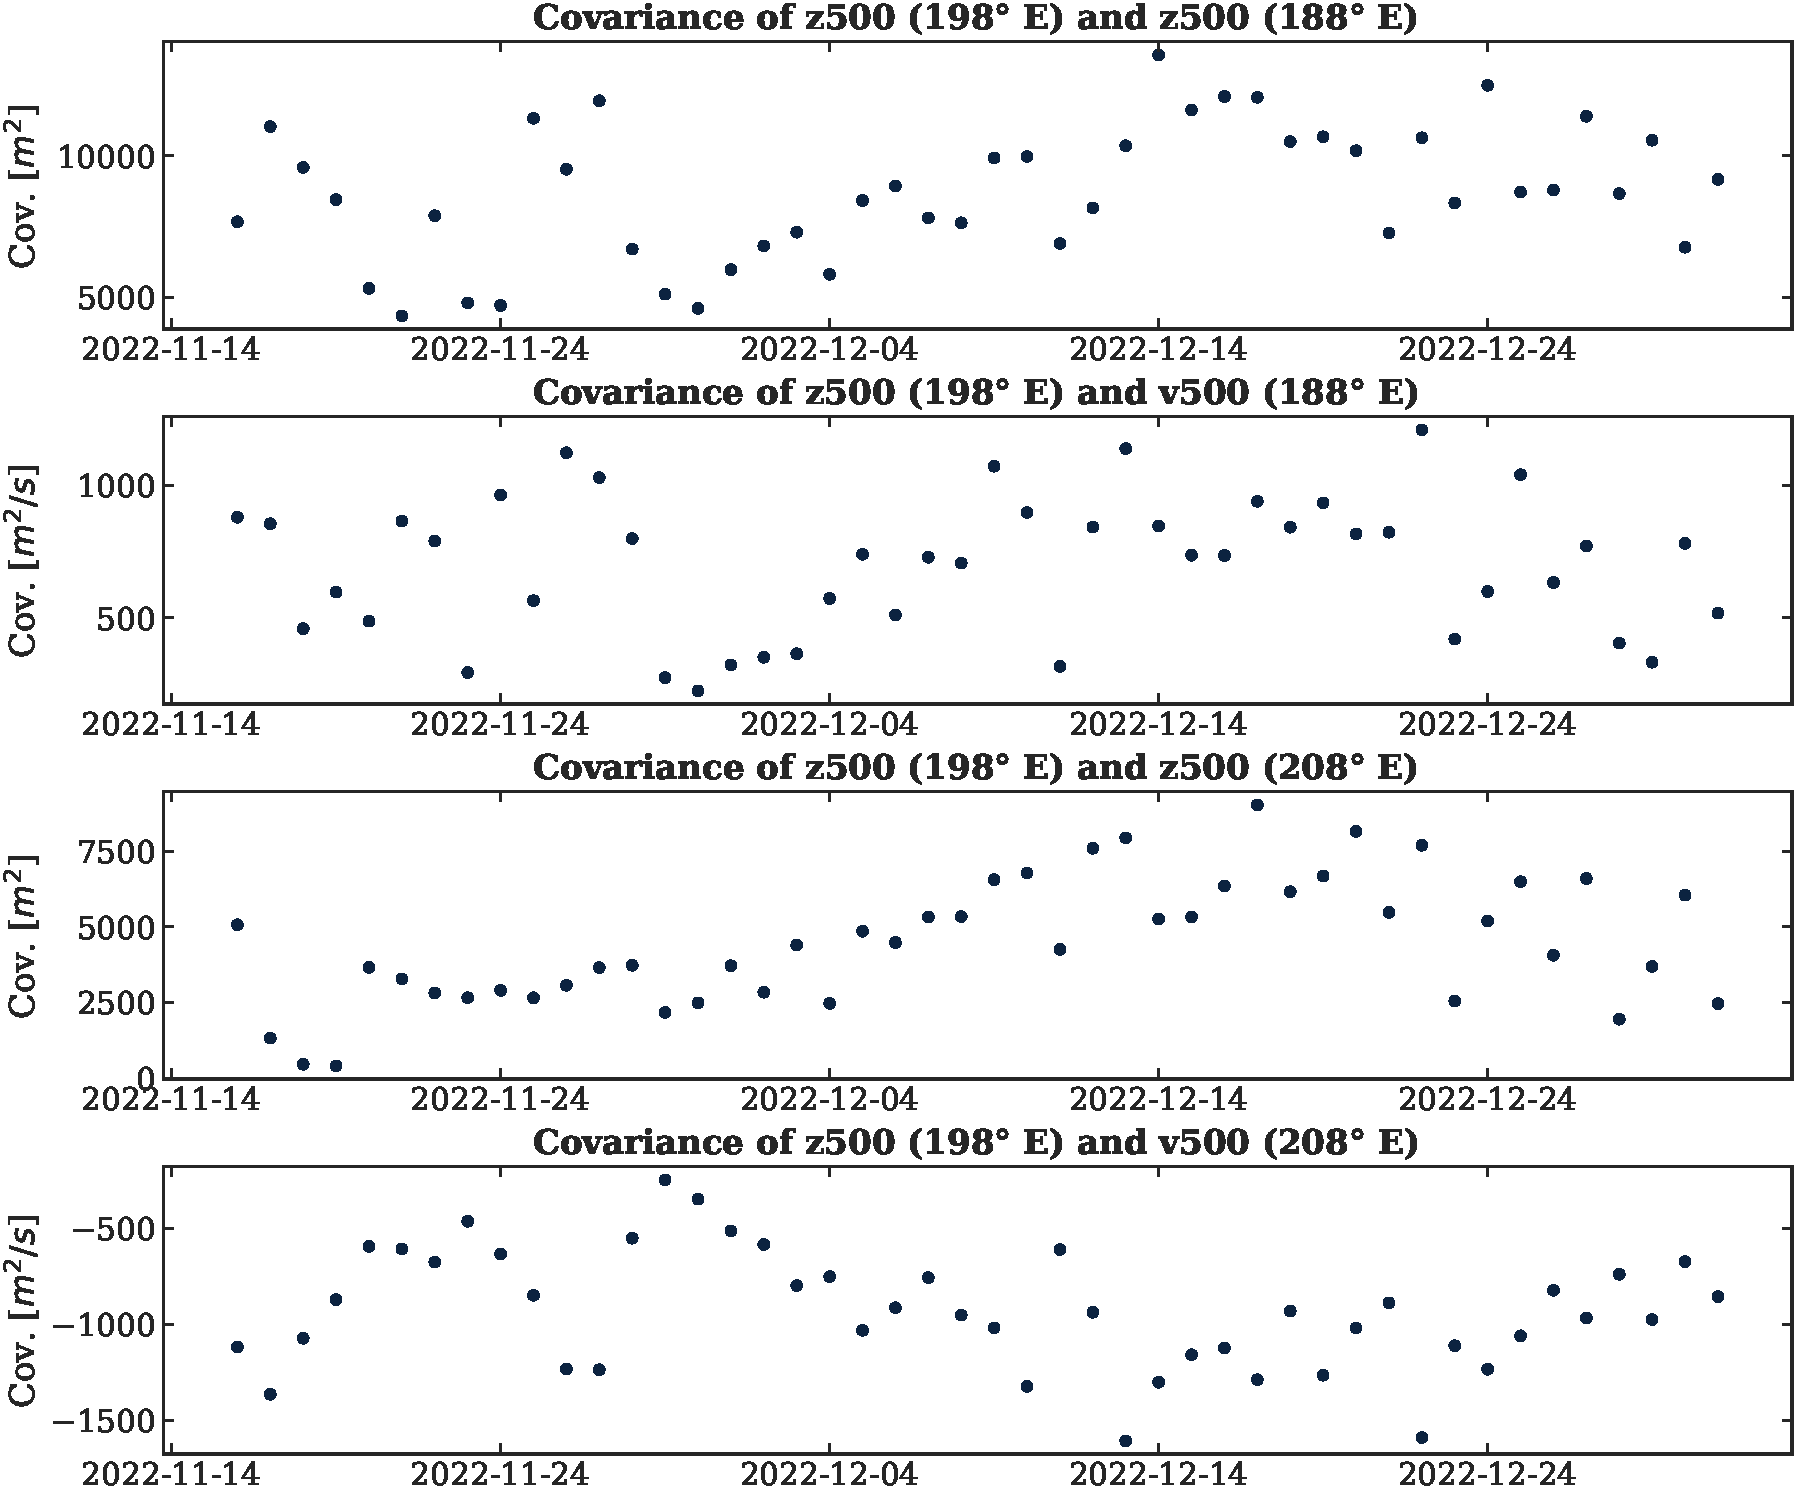
\includegraphics[width=\textwidth]{figures/cov.pdf}
   \caption{Sample covariance from the prior between fields and locations.}
   \label{fig:covs}
\end{figure}

Time series of the sample covariances at the three locations are shown in \cref{fig:covs}. The covariances change with time, but it appears to be a random walk rather than a physically meaningful change. There is a minimum in most of the absolute covariances around December 1. The meriodinal wind speeds have covariances of opposite signs with the geopotential height in between, as postulated by geostrophic flow.



\newpage
\section{Geopotential height}

\begin{figure}[ht]
   \centering

   \begin{subfigure}[c]{\textwidth}
      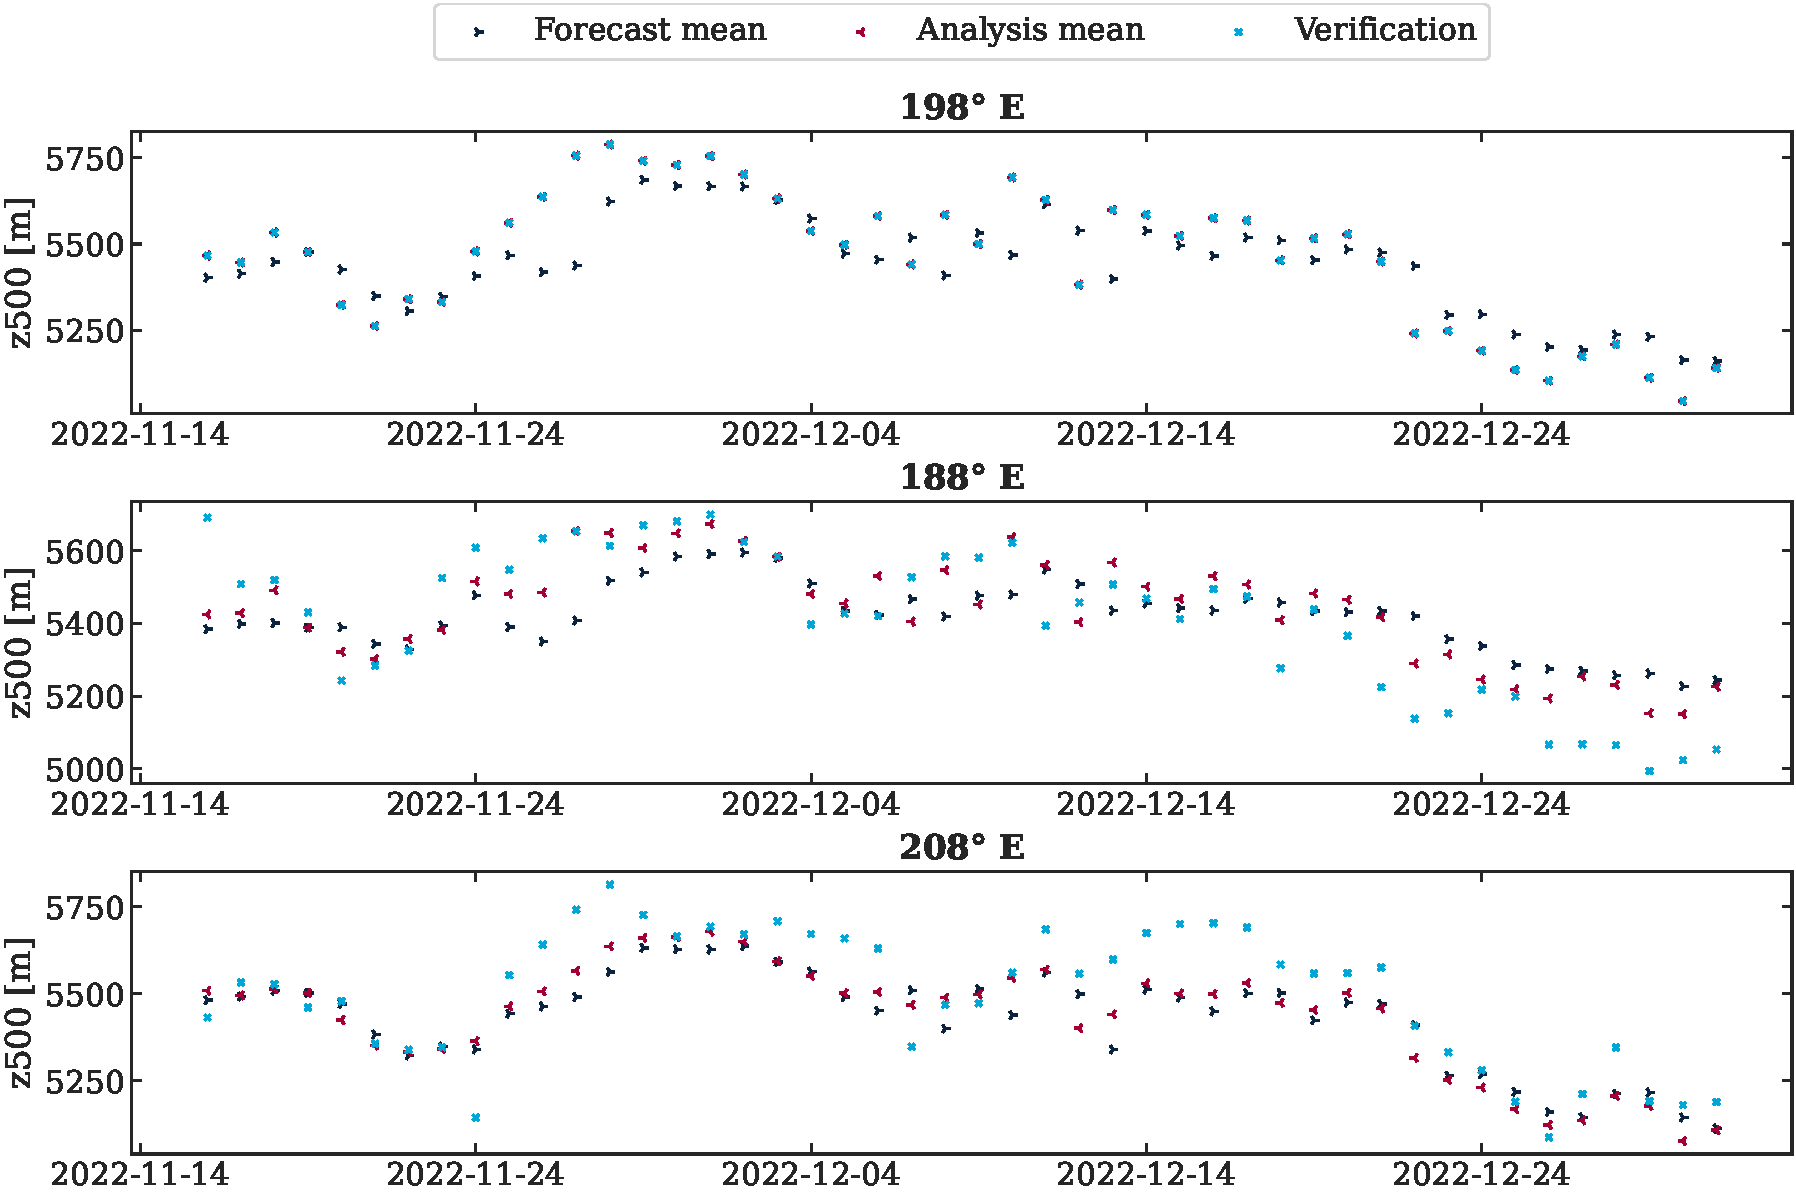
\includegraphics[width=\textwidth]{figures/height_means.pdf}
      \subcaption{Ensemble mean}
   \end{subfigure}
    
   \bigskip
    
   \begin{subfigure}[c]{\textwidth}
      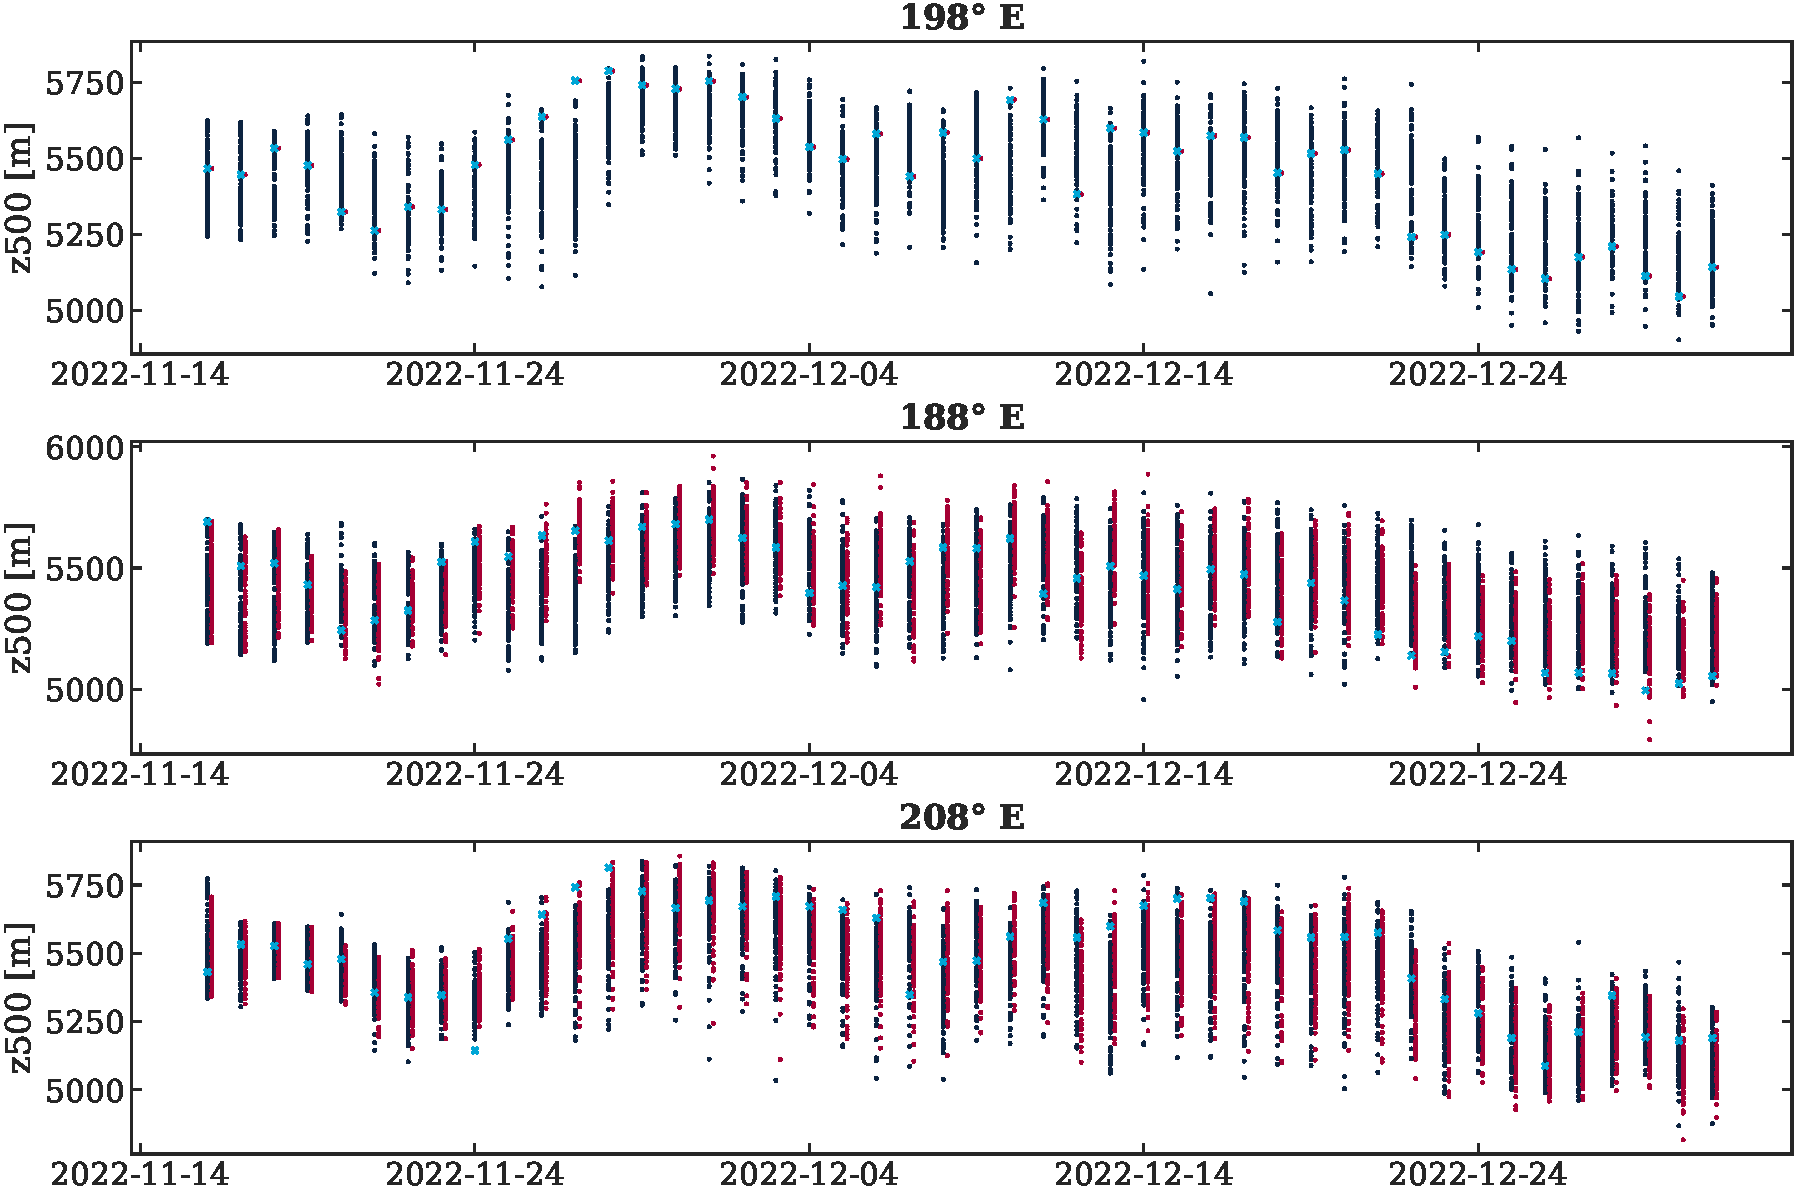
\includegraphics[width=\textwidth]{figures/heights.pdf}
      \subcaption{Ensemble samples}
   \end{subfigure}

   \caption{Geopotential height.}
   \label{fig:height}
\end{figure}

Time series of the geopotential height at the three locations are shown in \cref{fig:height}.
At the observation location, the analysis always coincides with the verification (which is identical to the observation for this location) since the state--observation covariance here is, obviously, maximal (correlation of 1). Therefore, the analysis spread is almost zero (exactly zero is prevented by the finite observation variance).
At the other locations, the analysis is generally closer to the observation than the prior, although this is not always the case. The analysis spread is generally slightly less than the prior spread, but not by much. In some cases (e.g., \ang{188} E on the third last day), the minimum--to--maximum range is even larger in the analysis, although the variance has to be smaller than that of the forecast by virtue of the EnSRF equations.
The ensemble spread remains relatively constant over time because it is reduced in the analysis but bumped in the forecast (emulating the $+Q$ term of the non-ensemble Kalman filter).

The ensemble variance and mean squared error (both for the forecast) are shown in \cref{fig:error}. The ensemble variance appears to be a lower bound for the true error, but usually underestimates it slightly, and in some cases dramatically.



\begin{figure}[h]
   \centering
   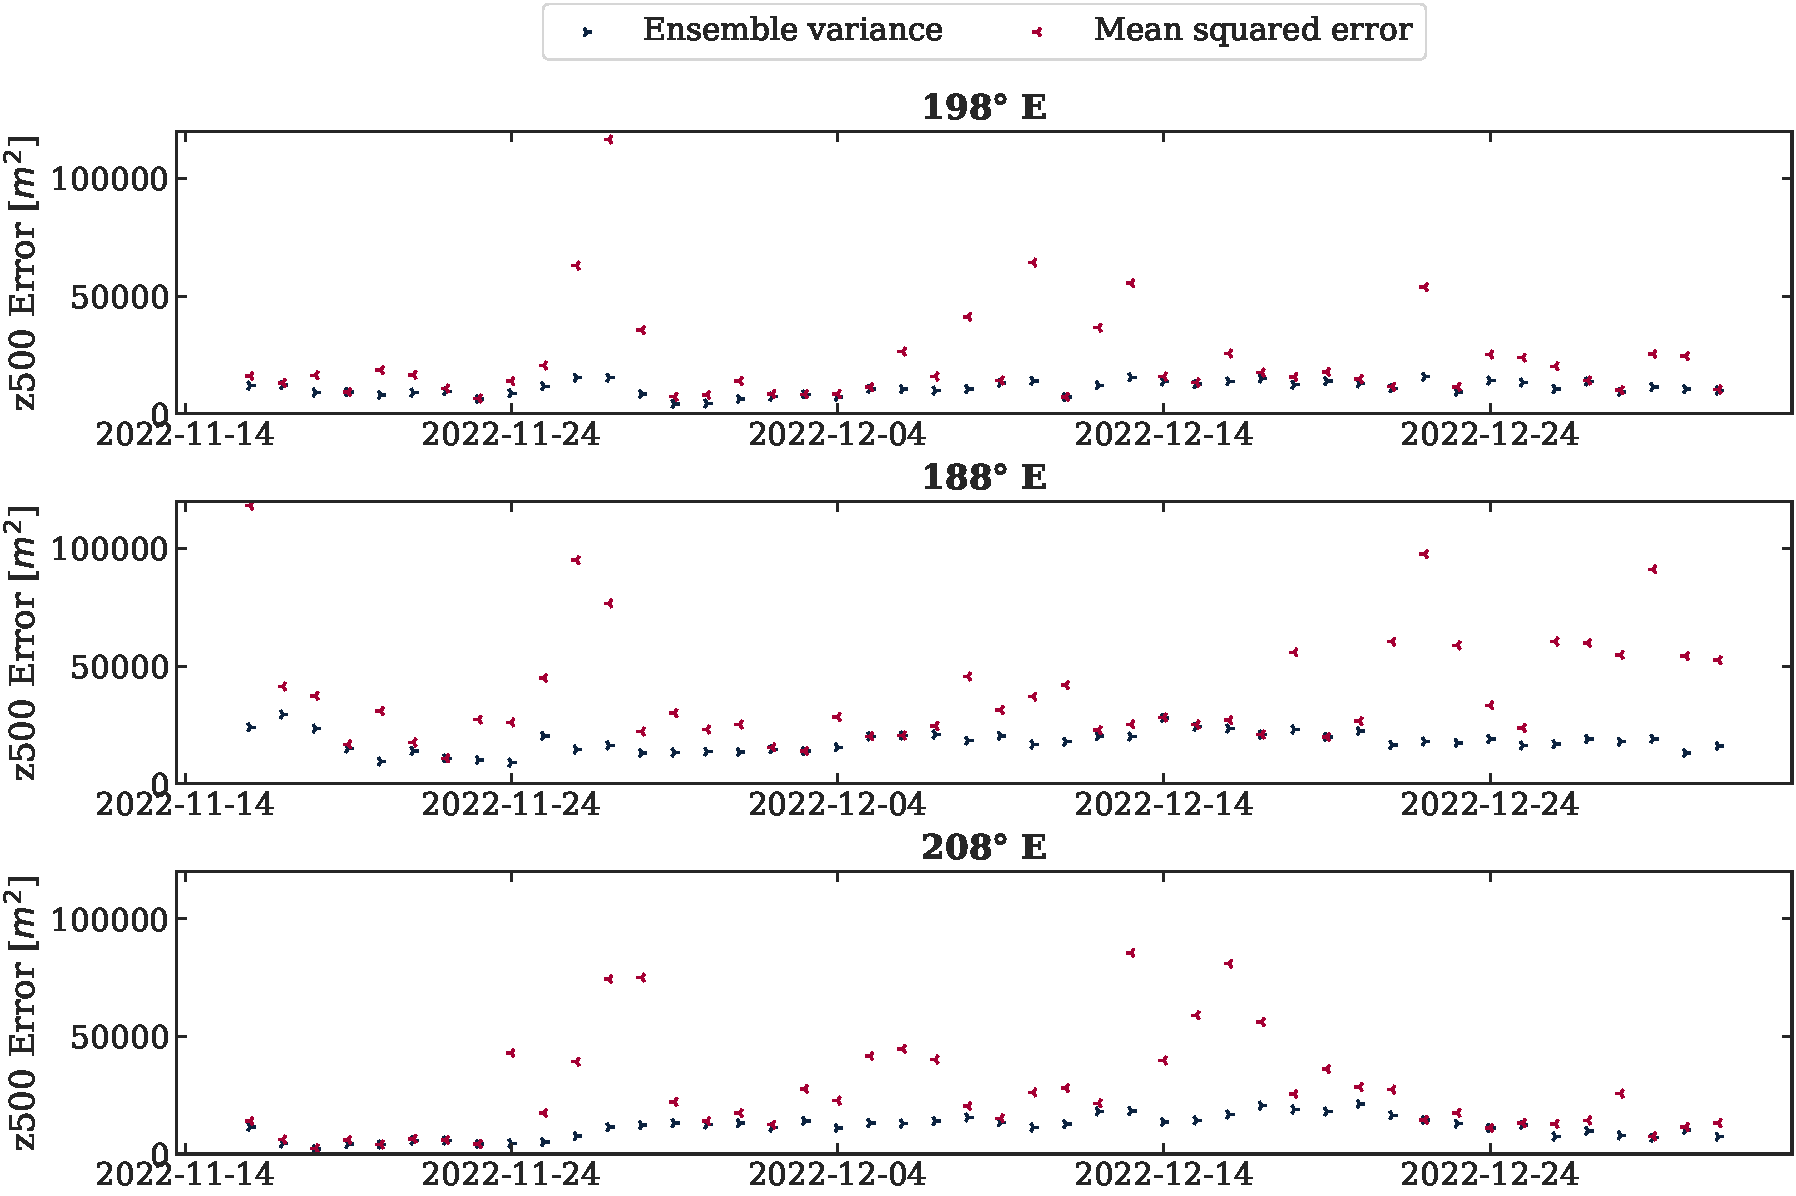
\includegraphics[width=\textwidth]{figures/height_error.pdf}
   \caption{Ensemble variance and mean squared error for geopotential height forecast.}
   \label{fig:error}
\end{figure}


\end{document}
